\vspace{0.8cm}

\noindent \textbf{\Large Avaliação Escrita 01 — Revisão Acelerada de Programação (RAP)}

\vspace{0.3cm}
\noindent \textbf{Orientações e Instruções para a Realização da Prova:}
\begin{itemize}[leftmargin=*]
    \item Esta avaliação é composta por \textbf{10 questões regulares} (totalizando \textbf{100,0 pontos}) e \textbf{1 Questão Bônus Especial} (valendo até \textbf{20,0 pontos extras}).
    \item \textbf{Estrutura da Prova:}
    \begin{itemize}
        \item \textbf{Parte I (Questões 1 a 7):} 7 Questões de Múltipla Escolha (Total: \textbf{30,0 pontos}).
        \item \textbf{Parte II (Questões 8 a 10):} 3 Questões Discursivas e de Programação em Python (Total: \textbf{70,0 pontos}).
        \item \textbf{Parte III (Questão 11):} 1 Questão Bônus de Simulação de Algoritmo em Python (\textbf{20,0 pontos extras}).
    \end{itemize}
    \item \textbf{Critérios de Correção e Resolução:}
    \begin{itemize}
        \item Nas questões de múltipla escolha, assinale com clareza a alternativa correta no espaço indicado.
        \item Nas questões discursivas, escreva o código Python de forma legível respeitando a indentação obrigatória, nomes de funções e parâmetros indicados nos protótipos.
        \item É proibido o uso de módulos externos não autorizados (utilize apenas funções nativas do Python).
    \end{itemize}
    \item \textbf{Tabela de Consulta (Anexo):} Ao final da prova, há uma tabela de referência rápida contendo a sintaxe e exemplos de funções e métodos nativos do Python que podem ser consultados livremente.
\end{itemize}

\vspace{0.4cm}

\section*{Parte I: Questões de Múltipla Escolha (Q1 a Q7 — 30,0 Pontos)}

\begin{enumerate}[label=\textbf{Q\arabic*.}, start=1]

% Q1 - 4,0 pontos (Copiada da Lista 11 Q1)
\item \textbf{[Múltipla Escolha - 4,0 pontos]} Considere a seguinte expressão aritmética executada em Python para calcular o valor total de uma compra com desconto:
\begin{minted}{python}
total = 10 + 2 * 3 ** 2 - 8 // 4 + 7 % 3
\end{minted}
Qual será o valor final atribuído à variável \code{total}?

\begin{itemize}[leftmargin=*]
    \item \textbf{Dica:} A ordem de precedência dos operadores aritméticos em Python é: 1º Parênteses \code{()}, 2º Exponenciação \code{**}, 3º Multiplicação \code{*}, Divisão \code{/}, Divisão Inteira \code{//} e Módulo \code{\%} (avaliados da esquerda para a direita), 4º Adição \code{+} e Subtração \code{-} (avaliados da esquerda para a direita). O operador de divisão inteira \code{//} retorna apenas a parte inteira da divisão (ex: \code{8 // 4} resulta em \code{2}), enquanto o operador módulo \code{\%} calcula o resto da divisão inteira (ex: \code{7 \% 3} resulta em \code{1}).
\end{itemize}

\begin{enumerate}[label=\textbf{(\Alph*)}]
    \item 25
    \item 27
    \item 28
    \item 30
    \item 19
\end{enumerate}

\ifmostrarGabarito
\textbf{Resposta: (B)}

\textbf{Justificativa:}
A ordem de precedência dos operadores aritméticos em Python é:
1. Exponenciação: $3 ** 2 = 9$
2. Multiplicação, divisão inteira e módulo (avaliados da esquerda para a direita):
   $2 * 9 = 18$, $8 // 4 = 2$, $7 \% 3 = 1$
3. Adição e subtração:
   $10 + 18 - 2 + 1 = 28 - 2 + 1 = 27$.
\else
\par\vspace{0.15cm}
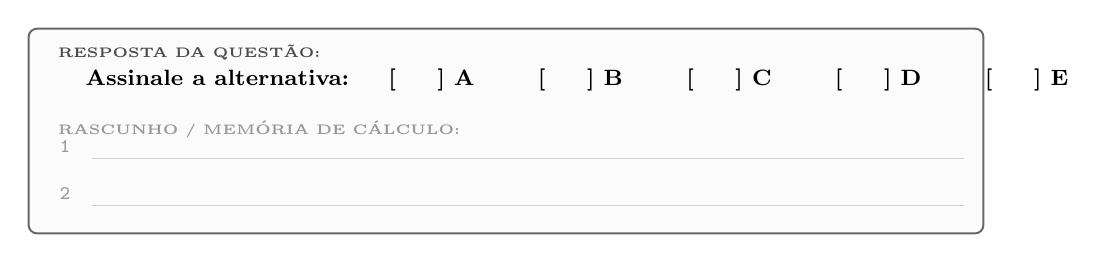
\begin{tikzpicture}
  \draw[rounded corners=3pt, draw=black!60, line width=0.7pt, fill=gray!3] (0,0) rectangle (\linewidth, -2.6cm);
  \node[anchor=north west, font=\tiny\bfseries\color{black!70}] at (0.25cm, -0.08cm) {RESPOSTA DA QUESTÃO:};
  \node[anchor=west, font=\footnotesize\bfseries] at (0.6cm, -0.65cm) {Assinale a alternativa: \quad [ \hspace{0.3cm} ] A \qquad [ \hspace{0.3cm} ] B \qquad [ \hspace{0.3cm} ] C \qquad [ \hspace{0.3cm} ] D \qquad [ \hspace{0.3cm} ] E};
  \node[anchor=north west, font=\tiny\bfseries\color{gray!80}] at (0.25cm, -1.05cm) {RASCUNHO / MEMÓRIA DE CÁLCULO:};
  \draw[gray!35, line width=0.4pt] (0.8cm, -1.65cm) -- (\linewidth-0.25cm, -1.65cm);
  \draw[gray!35, line width=0.4pt] (0.8cm, -2.25cm) -- (\linewidth-0.25cm, -2.25cm);
  \node[anchor=east, font=\scriptsize\ttfamily\color{gray!80}] at (0.65cm, -1.5cm) {1};
  \node[anchor=east, font=\scriptsize\ttfamily\color{gray!80}] at (0.65cm, -2.1cm) {2};
\end{tikzpicture}
\par\vspace{0.2cm}
\fi


\vspace{0.4cm}

% Q2 - 4,0 pontos (Copiada da Lista 11 Q11)
\item \textbf{[Múltipla Escolha - 4,0 pontos]} Em Python, a avaliação de expressões lógicas com os operadores \code{and} e \code{or} segue a regra do curto-circuito (\emph{short-circuit evaluation}). Considere as variáveis:
\begin{minted}{python}
x = 0
y = 10
z = 20
\end{minted}
Analise a expressão lógica:
\begin{minted}{python}
resultado = (x != 0 and (y / x) > 2) or (z > y and y > 0)
\end{minted}
Qual é o valor final atribuído a \code{resultado} e qual comportamento ocorre durante a execução?

\begin{itemize}[leftmargin=*]
    \item \textbf{Dica:} Na avaliação de curto-circuito (\emph{short-circuit evaluation}), o interpretador Python interrompe a avaliação de uma expressão lógica assim que o valor final já pode ser determinado:
    \begin{itemize}
        \item No operador \code{and}, se o primeiro termo for falso (\code{False}), o segundo termo \textbf{não é avaliado}, pois toda a conjunção será necessariamente falsa.
        \item No operador \code{or}, se o primeiro termo for verdadeiro (\code{True}), o segundo termo \textbf{não é avaliado}. Se o primeiro termo for falso, o segundo termo é avaliado para definir o resultado final.
    \end{itemize}
\end{itemize}


\begin{enumerate}[label=\textbf{(\Alph*)}]
    \item Ocorre um erro de divisão por zero (\code{ZeroDivisionError}) ao tentar avaliar \code{y / x}.
    \item O valor é \code{True}, pois a primeira parte da conjunção \code{x != 0} é \code{False}, evitando a divisão por zero, e a segunda parte do \code{or} é \code{True}.
    \item O valor é \code{False}, pois a primeira expressão é falsa e invalida todo o teste lógico.
    \item O valor é \code{None}, pois expressões com curto-circuito em Python não retornam valores booleanos puros.
    \item O programa trava em um laço infinito aguardando a definição do operador de curto-circuito.
\end{enumerate}

\ifmostrarGabarito
\textbf{Resposta: (B)}

\textbf{Justificativa:}
Em Python, na expressão \texttt{(x != 0 and (y / x) > 2)}, o termo \texttt{x != 0} é \texttt{False}. Pela regra do curto-circuito do operador \texttt{and}, a segunda parte \texttt{(y / x) > 2} nunca é executada, evitando o erro de divisão por zero.
Em seguida, o operador \texttt{or} avalia o lado direito: \texttt{(z > y and y > 0)}, que resulta em \texttt{(20 > 10 and 10 > 0) -> True and True -> True}. Logo, o resultado final é \texttt{True}.
\else
\par\vspace{0.15cm}
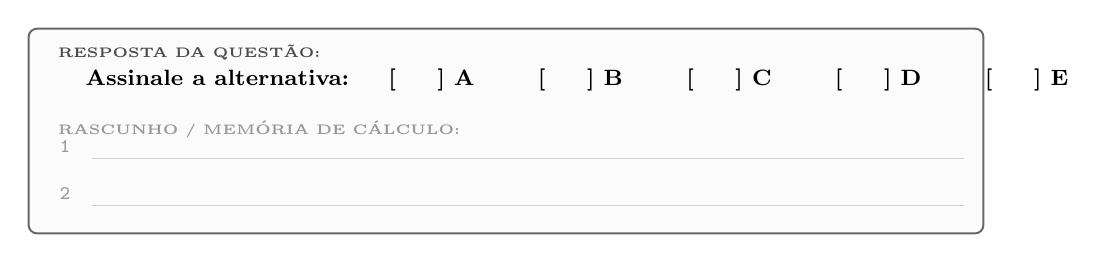
\begin{tikzpicture}
  \draw[rounded corners=3pt, draw=black!60, line width=0.7pt, fill=gray!3] (0,0) rectangle (\linewidth, -2.6cm);
  \node[anchor=north west, font=\tiny\bfseries\color{black!70}] at (0.25cm, -0.08cm) {RESPOSTA DA QUESTÃO:};
  \node[anchor=west, font=\footnotesize\bfseries] at (0.6cm, -0.65cm) {Assinale a alternativa: \quad [ \hspace{0.3cm} ] A \qquad [ \hspace{0.3cm} ] B \qquad [ \hspace{0.3cm} ] C \qquad [ \hspace{0.3cm} ] D \qquad [ \hspace{0.3cm} ] E};
  \node[anchor=north west, font=\tiny\bfseries\color{gray!80}] at (0.25cm, -1.05cm) {RASCUNHO / MEMÓRIA DE CÁLCULO:};
  \draw[gray!35, line width=0.4pt] (0.8cm, -1.65cm) -- (\linewidth-0.25cm, -1.65cm);
  \draw[gray!35, line width=0.4pt] (0.8cm, -2.25cm) -- (\linewidth-0.25cm, -2.25cm);
  \node[anchor=east, font=\scriptsize\ttfamily\color{gray!80}] at (0.65cm, -1.5cm) {1};
  \node[anchor=east, font=\scriptsize\ttfamily\color{gray!80}] at (0.65cm, -2.1cm) {2};
\end{tikzpicture}
\par\vspace{0.2cm}
\fi


\vspace{0.4cm}

% Q3 - 4,0 pontos (Copiada da Lista 11 Q31)
\item \textbf{[Múltipla Escolha - 4,0 pontos]} Dada a string \code{s = "PROGRAMACAO"}, qual será o resultado da operação de fatiamento \code{s[1:8:2]}?

\begin{enumerate}[label=\textbf{(\Alph*)}]
    \item \code{"RMAA"}
    \item \code{"RGAA"}
    \item \code{"RGA"}
    \item \code{"PGMC"}
    \item \code{"ROAM"}
\end{enumerate}

\ifmostrarGabarito
\textbf{Resposta: (B)}

\textbf{Justificativa:}
Os índices da string \code{"PROGRAMACAO"} (tamanho 11) são:
\texttt{P(0), R(1), O(2), G(3), R(4), A(5), M(6), A(7), C(8), A(9), O(10)}.

A operação de fatiamento \code{s[1:8:2]} seleciona os elementos a partir do índice de início 1 até antes do índice de parada 8, com passo 2:
\begin{itemize}
    \item Índice 1: \code{'R'}
    \item Índice 3: \code{'G'}
    \item Índice 5: \code{'A'}
    \item Índice 7: \code{'A'}
\end{itemize}
Concatenando os caracteres selecionados, o resultado é \code{"RGAA"}.
\else
\par\vspace{0.15cm}
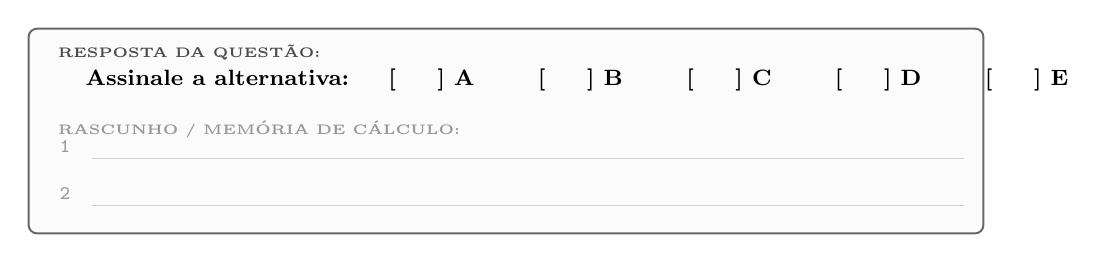
\begin{tikzpicture}
  \draw[rounded corners=3pt, draw=black!60, line width=0.7pt, fill=gray!3] (0,0) rectangle (\linewidth, -2.6cm);
  \node[anchor=north west, font=\tiny\bfseries\color{black!70}] at (0.25cm, -0.08cm) {RESPOSTA DA QUESTÃO:};
  \node[anchor=west, font=\footnotesize\bfseries] at (0.6cm, -0.65cm) {Assinale a alternativa: \quad [ \hspace{0.3cm} ] A \qquad [ \hspace{0.3cm} ] B \qquad [ \hspace{0.3cm} ] C \qquad [ \hspace{0.3cm} ] D \qquad [ \hspace{0.3cm} ] E};
  \node[anchor=north west, font=\tiny\bfseries\color{gray!80}] at (0.25cm, -1.05cm) {RASCUNHO / MEMÓRIA DE CÁLCULO:};
  \draw[gray!35, line width=0.4pt] (0.8cm, -1.65cm) -- (\linewidth-0.25cm, -1.65cm);
  \draw[gray!35, line width=0.4pt] (0.8cm, -2.25cm) -- (\linewidth-0.25cm, -2.25cm);
  \node[anchor=east, font=\scriptsize\ttfamily\color{gray!80}] at (0.65cm, -1.5cm) {1};
  \node[anchor=east, font=\scriptsize\ttfamily\color{gray!80}] at (0.65cm, -2.1cm) {2};
\end{tikzpicture}
\par\vspace{0.2cm}
\fi


\vspace{0.4cm}

% Q4 - 4,0 pontos (Copiada da Lista 11 Q42)
\item \textbf{[Múltipla Escolha - 4,0 pontos]} Em Python, a atribuição direta entre variáveis que apontam para listas cria uma referência (\emph{alias}), enquanto o método \code{.copy()} ou o fatiamento \texttt{[:]} cria uma cópia rasa (\emph{shallow copy}). Analise o código abaixo:
\begin{minted}{python}
lista_a = [10, 20, 30]
lista_b = lista_a
lista_c = lista_a.copy()

lista_b.append(40)
lista_c.append(50)
\end{minted}
Quais serão os valores finais de \code{lista\_a}, \code{lista\_b} e \code{lista\_c}, respectivamente?

\begin{enumerate}[label=\textbf{(\Alph*)}]
    \item \texttt{[10, 20, 30]}, \texttt{[10, 20, 30, 40]} e \texttt{[10, 20, 30, 50]}
    \item \texttt{[10, 20, 30, 40, 50]}, \texttt{[10, 20, 30, 40, 50]} e \texttt{[10, 20, 30, 50]}
    \item \texttt{[10, 20, 30]}, \texttt{[10, 20, 30, 40]} e \texttt{[10, 20, 30]}
    \item \texttt{[10, 20, 30, 40]}, \texttt{[10, 20, 30, 40]} e \texttt{[10, 20, 30, 50]}
    \item \texttt{[10, 20, 30, 50]}, \texttt{[10, 20, 30, 40]} e \texttt{[10, 20, 30, 50]}
\end{enumerate}

\ifmostrarGabarito
\textbf{Resposta: (D)}

\textbf{Justificativa:}
Como \texttt{lista\_b = lista\_a}, ambas as variáveis apontam para o mesmo objeto na memória. Portanto, a alteração \texttt{lista\_b.append(40)} afeta tanto \texttt{lista\_b} quanto \texttt{lista\_a}.
Já \texttt{lista\_c = lista\_a.copy()} cria uma nova lista independente contendo os mesmos elementos originais \texttt{[10, 20, 30]}. A alteração \texttt{lista\_c.append(50)} afeta exclusivamente \texttt{lista\_c}.
Resultados finais:
- \texttt{lista\_a = [10, 20, 30, 40]}
- \texttt{lista\_b = [10, 20, 30, 40]}
- \texttt{lista\_c = [10, 20, 30, 50]}
\else
\par\vspace{0.15cm}
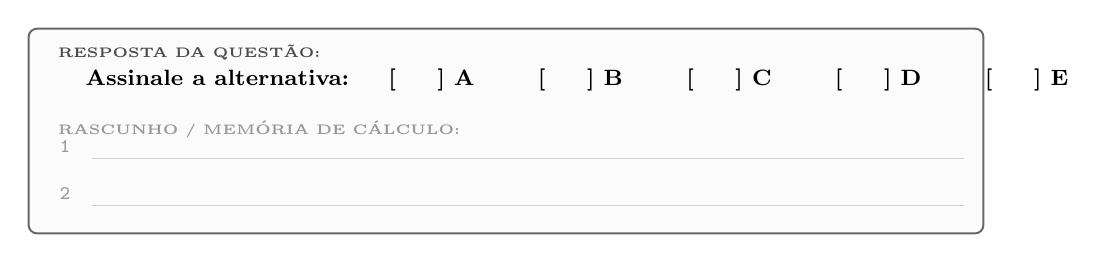
\begin{tikzpicture}
  \draw[rounded corners=3pt, draw=black!60, line width=0.7pt, fill=gray!3] (0,0) rectangle (\linewidth, -2.6cm);
  \node[anchor=north west, font=\tiny\bfseries\color{black!70}] at (0.25cm, -0.08cm) {RESPOSTA DA QUESTÃO:};
  \node[anchor=west, font=\footnotesize\bfseries] at (0.6cm, -0.65cm) {Assinale a alternativa: \quad [ \hspace{0.3cm} ] A \qquad [ \hspace{0.3cm} ] B \qquad [ \hspace{0.3cm} ] C \qquad [ \hspace{0.3cm} ] D \qquad [ \hspace{0.3cm} ] E};
  \node[anchor=north west, font=\tiny\bfseries\color{gray!80}] at (0.25cm, -1.05cm) {RASCUNHO / MEMÓRIA DE CÁLCULO:};
  \draw[gray!35, line width=0.4pt] (0.8cm, -1.65cm) -- (\linewidth-0.25cm, -1.65cm);
  \draw[gray!35, line width=0.4pt] (0.8cm, -2.25cm) -- (\linewidth-0.25cm, -2.25cm);
  \node[anchor=east, font=\scriptsize\ttfamily\color{gray!80}] at (0.65cm, -1.5cm) {1};
  \node[anchor=east, font=\scriptsize\ttfamily\color{gray!80}] at (0.65cm, -2.1cm) {2};
\end{tikzpicture}
\par\vspace{0.2cm}
\fi


\vspace{0.4cm}

% Q5 - 4,0 pontos (Processamento de Strings com split e join)
\item \textbf{[Múltipla Escolha - 4,0 pontos]} Considere a seguinte rotina em Python utilizada para higienização e formatação de um registro de texto:
\begin{minted}{python}
registro = "  joao ; silva ; 1995 ; engenheiro  "
partes = [campo.strip().upper() for campo in registro.split(";")]
resultado = " - ".join(partes[:2])
\end{minted}
Qual será o valor exato atribuído à variável \code{resultado} ao final da execução?

\begin{enumerate}[label=\textbf{(\Alph*)}]
    \item \code{"JOAO - SILVA"}
    \item \code{"JOAO ; SILVA"}
    \item \code{"JOAO - SILVA - 1995"}
    \item \code{"  JOAO   -   SILVA  "}
    \item \code{['JOAO', 'SILVA']}
\end{enumerate}

\ifmostrarGabarito
\textbf{Resposta: (A)}

\textbf{Justificativa:}
Passo a passo da execução do código:
\begin{enumerate}
    \item \code{registro.split(";")} divide a string pelo caractere delimitador \code{";"}, gerando a lista:
    \texttt{["  joao ", " silva ", " 1995 ", " engenheiro  "]}.
    \item A compreensão de lista aplica \code{.strip().upper()} a cada elemento:
    \begin{itemize}
        \item \code{.strip()} remove todos os espaços em branco iniciais e finais;
        \item \code{.upper()} converte todas as letras para caixa alta;
    \end{itemize}
    resultando na lista: \texttt{['JOAO', 'SILVA', '1995', 'ENGENHEIRO']}.
    \item O fatiamento \code{partes[:2]} seleciona os dois primeiros elementos (índices 0 e 1): \texttt{['JOAO', 'SILVA']}.
    \item O método \code{" - ".join(...)} concatena os elementos da fatia intercalados pelo delimitador \code{" - "}, produzindo a string final: \code{"JOAO - SILVA"}.
\end{enumerate}
\else
\par\vspace{0.15cm}
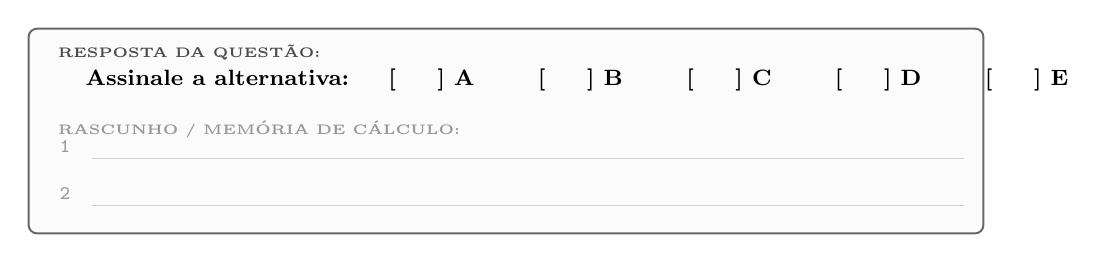
\begin{tikzpicture}
  \draw[rounded corners=3pt, draw=black!60, line width=0.7pt, fill=gray!3] (0,0) rectangle (\linewidth, -2.6cm);
  \node[anchor=north west, font=\tiny\bfseries\color{black!70}] at (0.25cm, -0.08cm) {RESPOSTA DA QUESTÃO:};
  \node[anchor=west, font=\footnotesize\bfseries] at (0.6cm, -0.65cm) {Assinale a alternativa: \quad [ \hspace{0.3cm} ] A \qquad [ \hspace{0.3cm} ] B \qquad [ \hspace{0.3cm} ] C \qquad [ \hspace{0.3cm} ] D \qquad [ \hspace{0.3cm} ] E};
  \node[anchor=north west, font=\tiny\bfseries\color{gray!80}] at (0.25cm, -1.05cm) {RASCUNHO / MEMÓRIA DE CÁLCULO:};
  \draw[gray!35, line width=0.4pt] (0.8cm, -1.65cm) -- (\linewidth-0.25cm, -1.65cm);
  \draw[gray!35, line width=0.4pt] (0.8cm, -2.25cm) -- (\linewidth-0.25cm, -2.25cm);
  \node[anchor=east, font=\scriptsize\ttfamily\color{gray!80}] at (0.65cm, -1.5cm) {1};
  \node[anchor=east, font=\scriptsize\ttfamily\color{gray!80}] at (0.65cm, -2.1cm) {2};
\end{tikzpicture}
\par\vspace{0.2cm}
\fi


\vspace{0.4cm}

% Q6 - 5,0 pontos (Nova Questão - Escopo & Funções)
\item \textbf{[Múltipla Escolha - 5,0 pontos]} Analise a execução do seguinte trecho de código em Python envolvendo escopo de variáveis e funções:
\begin{minted}{python}
taxa = 1.10

def atualizar_precos(valores: list[float]) -> float:
    global taxa
    taxa = 1.20
    soma = 0.0
    for i in range(len(valores)):
        valores[i] = valores[i] * taxa
        soma += valores[i]
    return soma

precos = [10.0, 20.0]
total_calculado = atualizar_precos(precos)
\end{minted}
Após a execução completa, quais serão os valores de \code{precos}, \code{total\_calculado} e da variável global \code{taxa}?

\begin{enumerate}[label=\textbf{(\Alph*)}]
    \item \texttt{precos = [10.0, 20.0]}, \texttt{total\_calculado = 33.0} e \texttt{taxa = 1.10}
    \item \texttt{precos = [12.0, 24.0]}, \texttt{total\_calculado = 36.0} e \texttt{taxa = 1.20}
    \item \texttt{precos = [11.0, 22.0]}, \texttt{total\_calculado = 33.0} e \texttt{taxa = 1.20}
    \item \texttt{precos = [12.0, 24.0]}, \texttt{total\_calculado = 36.0} e \texttt{taxa = 1.10}
    \item Ocorre um erro de compilação (\texttt{UnboundLocalError}) devido ao uso de \texttt{global taxa}.
\end{enumerate}

\ifmostrarGabarito
\textbf{Resposta: (B)}

\textbf{Justificativa:}
1. O comando \texttt{global taxa} declara que a função modificará a variável global \texttt{taxa}, atribuindo-lhe o novo valor \texttt{1.20}.
2. Como listas são objetos mutáveis passados por referência, a modificação \texttt{valores[i] = valores[i] * 1.20} altera diretamente os elementos da lista \texttt{precos}:
   - $10.0 \times 1.20 = 12.0$
   - $20.0 \times 1.20 = 24.0$
   Portanto, \texttt{precos} torna-se \texttt{[12.0, 24.0]}.
3. O somatório retornado é $12.0 + 24.0 = 36.0$.
4. A variável global \texttt{taxa} foi atualizada para \texttt{1.20}.
\else
\par\vspace{0.15cm}
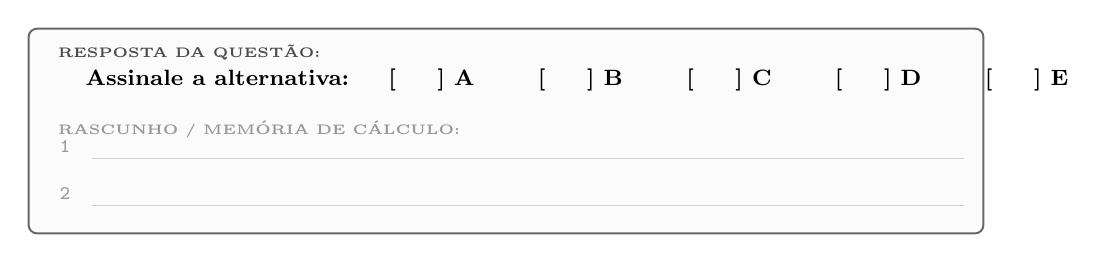
\begin{tikzpicture}
  \draw[rounded corners=3pt, draw=black!60, line width=0.7pt, fill=gray!3] (0,0) rectangle (\linewidth, -2.6cm);
  \node[anchor=north west, font=\tiny\bfseries\color{black!70}] at (0.25cm, -0.08cm) {RESPOSTA DA QUESTÃO:};
  \node[anchor=west, font=\footnotesize\bfseries] at (0.6cm, -0.65cm) {Assinale a alternativa: \quad [ \hspace{0.3cm} ] A \qquad [ \hspace{0.3cm} ] B \qquad [ \hspace{0.3cm} ] C \qquad [ \hspace{0.3cm} ] D \qquad [ \hspace{0.3cm} ] E};
  \node[anchor=north west, font=\tiny\bfseries\color{gray!80}] at (0.25cm, -1.05cm) {RASCUNHO / MEMÓRIA DE CÁLCULO:};
  \draw[gray!35, line width=0.4pt] (0.8cm, -1.65cm) -- (\linewidth-0.25cm, -1.65cm);
  \draw[gray!35, line width=0.4pt] (0.8cm, -2.25cm) -- (\linewidth-0.25cm, -2.25cm);
  \node[anchor=east, font=\scriptsize\ttfamily\color{gray!80}] at (0.65cm, -1.5cm) {1};
  \node[anchor=east, font=\scriptsize\ttfamily\color{gray!80}] at (0.65cm, -2.1cm) {2};
\end{tikzpicture}
\par\vspace{0.2cm}
\fi


\vspace{0.4cm}

% Q7 - 5,0 pontos (Nova Questão - POO)
\item \textbf{[Múltipla Escolha - 5,0 pontos]} Na Programação Orientada a Objetos em Python, considere o seguinte modelo de classes:
\begin{minted}{python}
class Sensor:
    def __init__(self, identificador: str):
        self.id = identificador
    
    def obter_status(self) -> str:
        return f"Sensor {self.id}: ATIVO"

class SensorSonar(Sensor):
    def __init__(self, identificador: str, profundidade_max: float):
        super().__init__(identificador)
        self.profundidade = profundidade_max
    
    def obter_status(self) -> str:
        msg_base = super().obter_status()
        return f"{msg_base} (Prof: {self.profundidade}m)"
\end{minted}
Ao instanciar \texttt{s = SensorSonar("SN-01", 300.0)} e executar \texttt{s.obter\_status()}, qual será o retorno produzido?

\begin{enumerate}[label=\textbf{(\Alph*)}]
    \item \texttt{"Sensor SN-01: ATIVO"}
    \item \texttt{"(Prof: 300.0m)"}
    \item Ocorre um erro de execução (\texttt{AttributeError}), pois \texttt{super()} não pode acessar métodos com o mesmo nome.
    \item \texttt{"Sensor SN-01: ATIVO (Prof: 300.0m)"}
    \item \texttt{"Sensor: None (Prof: 300.0m)"}
\end{enumerate}

\ifmostrarGabarito
\textbf{Resposta: (D)}

\textbf{Justificativa:}
A classe filha \texttt{SensorSonar} herda de \texttt{Sensor}.
1. No construtor \texttt{\_\_init\_\_}, \texttt{super().\_\_init\_\_(identificador)} inicializa o atributo herdado \texttt{self.id = "SN-01"}.
2. No método \texttt{obter\_status}, a chamada \texttt{super().obter\_status()} executa a versão da classe base, retornando \texttt{"Sensor SN-01: ATIVO"}.
3. O método concatena \texttt{" (Prof: 300.0m)"}, gerando a string completa: \texttt{"Sensor SN-01: ATIVO (Prof: 300.0m)"}.
\else
\par\vspace{0.15cm}
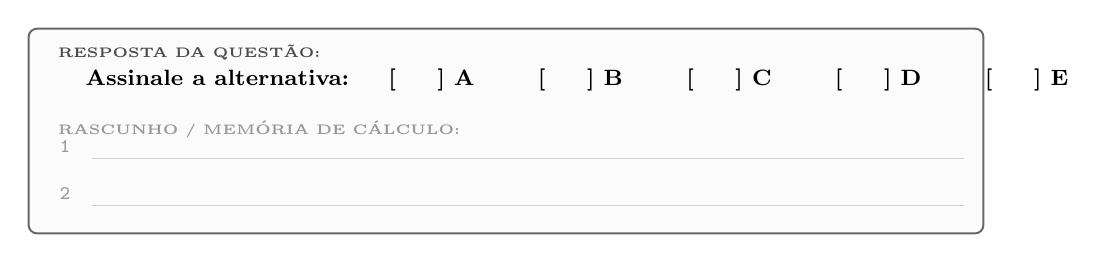
\begin{tikzpicture}
  \draw[rounded corners=3pt, draw=black!60, line width=0.7pt, fill=gray!3] (0,0) rectangle (\linewidth, -2.6cm);
  \node[anchor=north west, font=\tiny\bfseries\color{black!70}] at (0.25cm, -0.08cm) {RESPOSTA DA QUESTÃO:};
  \node[anchor=west, font=\footnotesize\bfseries] at (0.6cm, -0.65cm) {Assinale a alternativa: \quad [ \hspace{0.3cm} ] A \qquad [ \hspace{0.3cm} ] B \qquad [ \hspace{0.3cm} ] C \qquad [ \hspace{0.3cm} ] D \qquad [ \hspace{0.3cm} ] E};
  \node[anchor=north west, font=\tiny\bfseries\color{gray!80}] at (0.25cm, -1.05cm) {RASCUNHO / MEMÓRIA DE CÁLCULO:};
  \draw[gray!35, line width=0.4pt] (0.8cm, -1.65cm) -- (\linewidth-0.25cm, -1.65cm);
  \draw[gray!35, line width=0.4pt] (0.8cm, -2.25cm) -- (\linewidth-0.25cm, -2.25cm);
  \node[anchor=east, font=\scriptsize\ttfamily\color{gray!80}] at (0.65cm, -1.5cm) {1};
  \node[anchor=east, font=\scriptsize\ttfamily\color{gray!80}] at (0.65cm, -2.1cm) {2};
\end{tikzpicture}
\par\vspace{0.2cm}
\fi


\ifmostrarGabarito\else\clearpage\fi

\section*{Parte II: Questões Discursivas e de Programação (Q8 a Q10 — 70,0 Pontos)}

% Q8 - 20,0 pontos (Desconto Progressivo em E-Commerce)
\item \textbf{[Discursiva - 20,0 pontos]} Uma loja online aplica descontos promocionais progressivos no fechamento do carrinho de compras conforme o valor total bruto gasto pelo cliente:
\begin{itemize}[leftmargin=*]
    \item Compras de até R\$ 100,00: sem desconto (0\%).
    \item Compras de R\$ 100,01 a R\$ 300,00: \textbf{5\%} de desconto.
    \item Compras de R\$ 300,01 a R\$ 500,00: \textbf{10\%} de desconto.
    \item Compras acima de R\$ 500,00: \textbf{15\%} de desconto.
\end{itemize}
Escreva a função \code{calcular\_desconto\_compra} que receba o valor bruto da compra e retorne uma tupla \code{(valor\_desconto, valor\_final\_a\_pagar)}, com ambos os valores arredondados para duas casas decimais com \code{round(..., 2)}. Caso o valor informado seja menor ou igual a zero, a função deve retornar \code{(0.0, 0.0)}.

\begin{itemize}[leftmargin=*]
    \item \textbf{Protótipo:}\newline \code{from typing import Tuple}\\\code{def calcular\_desconto\_compra(}\\\code{    valor\_bruto: float}\\\code{) -> Tuple[float, float]:}
    \item \textbf{Exemplos de Teste:}\newline
    \code{calcular\_desconto\_compra(200.0)} $\rightarrow$ \code{(10.0, 190.0)}\newline
    \code{calcular\_desconto\_compra(400.0)} $\rightarrow$ \code{(40.0, 360.0)}\newline
    \code{calcular\_desconto\_compra(600.0)} $\rightarrow$ \code{(90.0, 510.0)}
\end{itemize}

\ifmostrarGabarito
\begin{minted}{python}
from typing import Tuple

def calcular_desconto_compra(valor_bruto: float) -> Tuple[float, float]:
    if valor_bruto <= 0:
        return (0.0, 0.0)
    
    if valor_bruto <= 100.0:
        taxa = 0.0
    elif valor_bruto <= 300.0:
        taxa = 0.05
    elif valor_bruto <= 500.0:
        taxa = 0.10
    else:
        taxa = 0.15
        
    desconto = round(valor_bruto * taxa, 2)
    valor_final = round(valor_bruto - desconto, 2)
    
    return (desconto, valor_final)
\end{minted}

\textbf{Explicação:}
A função valida inicialmente se a entrada é válida (estritamente positiva). Em seguida, aplica uma estrutura condicional (\texttt{if / elif / else}) para determinar a taxa de desconto conforme as faixas de valor especificadas, calculando o desconto e o valor líquido a pagar com arredondamento para duas casas decimais.

\vspace{0.3cm}
\textbf{Critérios de Correção e Penalidades Sugeridas (Erros Comuns):}
\begin{itemize}[leftmargin=*, noitemsep, topsep=2pt]
    \item \textbf{Validação de entrada nula ou negativa} (\textbf{--4,0 pontos}): Não tratar valores $\le 0$ retornando \code{(0.0, 0.0)}.
    \item \textbf{Lógica e faixas de desconto} (\textbf{--6,0 pontos}): Erro nas comparações de limites (ex.: usar operador estrito \code{<} em vez de \code{<=}) ou faixas invertidas.
    \item \textbf{Cálculo aritmético} (\textbf{--4,0 pontos}): Erro na multiplicação da taxa ou esquecer de subtrair o desconto do valor bruto.
    \item \textbf{Arredondamento} (\textbf{--3,0 pontos}): Não utilizar \code{round(..., 2)} no desconto ou no valor a pagar.
    \item \textbf{Formato de retorno} (\textbf{--3,0 pontos}): Retornar tipo incorreto (ex.: lista em vez de tupla) ou usar \code{print} em vez de \code{return}.
\end{itemize}
\else
\linhasResposta{18}
\clearpage
\linhasResposta[FOLHA DE CONTINUACAO / RASCUNHO -- QUESTAO Q8]{30}
\clearpage
\fi


\vspace{0.5cm}

% Q9 - 25,0 pontos (Laços & Modularização de Funções: Números Primos)
\item \textbf{[Discursiva - 25,0 pontos]} Um número natural maior do que 1 é dito \textbf{primo} se for divisível apenas por 1 e por ele mesmo (números $\le 1$ não são primos). Para resolver este problema de forma modular e aplicando boas práticas de programação, você deve implementar obrigatoriamente \textbf{duas funções}:

\begin{itemize}[leftmargin=*]
    \item \textbf{1. Função Auxiliar \code{eh\_primo(numero: int) -> bool}:}\newline
    Recebe um número inteiro e verifica se ele é primo utilizando laço de repetição e o operador módulo \code{\%}. Retorna \code{True} se o número for primo ou \code{False} caso contrário.
    \item \textbf{2. Função Principal \code{filtrar\_primos\_intervalo(inicio: int, fim: int) -> List[int]}:}\newline
    Recebe dois inteiros positivos \code{inicio} e \code{fim} ($\text{inicio} \le \text{fim}$). Esta função deve iterar pelos números do intervalo fechado $[\text{inicio}, \text{fim}]$ e \textbf{chamar obrigatoriamente a função auxiliar \code{eh\_primo}} para cada número, retornando uma \textbf{lista} contendo todos os números primos encontrados em ordem crescente. Caso não haja primos no intervalo, retorne uma lista vazia \code{[]}.
\end{itemize}

\begin{itemize}[leftmargin=*]
    \item \textbf{Dica:} Para verificar se um número $n$ é primo, basta testar se algum inteiro $d$ no intervalo $2 \le d \le \sqrt{n}$ divide $n$ de forma exata (\code{n \% d == 0}). Lembre-se de que números $\le 1$ não são primos.
    \item \textbf{Protótipos Obrigatórios:}\newline
    \code{def eh\_primo(numero: int) -> bool:}\newline
    \code{from typing import List}\newline
    \code{def filtrar\_primos\_intervalo(inicio: int, fim: int) -> List[int]:}
    \item \textbf{Exemplo de Teste:} \code{filtrar\_primos\_intervalo(10, 30)} $\rightarrow$ \code{[11, 13, 17, 19, 23, 29]}
\end{itemize}

\ifmostrarGabarito
\begin{minted}{python}
from typing import List

def eh_primo(numero: int) -> bool:
    if numero <= 1:
        return False
    for divisor in range(2, int(numero**0.5) + 1):
        if numero % divisor == 0:
            return False
    return True

def filtrar_primos_intervalo(inicio: int, fim: int) -> List[int]:
    primos = []
    for num in range(inicio, fim + 1):
        if eh_primo(num):
            primos.append(num)
    return primos
\end{minted}

\textbf{Explicação:}
A solução adota a modularização em duas funções:
\begin{enumerate}
    \item \texttt{eh\_primo}: Testa se um número individual é primo, descartando números $\le 1$ e verificando divisores até $\sqrt{\text{numero}}$.
    \item \texttt{filtrar\_primos\_intervalo}: Percorre o intervalo fechado de \texttt{inicio} a \texttt{fim}, chamando \texttt{eh\_primo(num)} para filtrar e acumular os números primos em uma lista.
\end{enumerate}

\vspace{0.3cm}
\textbf{Critérios de Correção e Penalidades Sugeridas (Erros Comuns):}
\begin{itemize}[leftmargin=*, noitemsep, topsep=2pt]
    \item \textbf{Falta de modularização ou não chamar função auxiliar} (\textbf{--6,0 pontos}): Implementar tudo em uma única função ou não invocar \code{eh\_primo} dentro de \code{filtrar\_primos\_intervalo}.
    \item \textbf{Falha nos casos base $\le 1$} (\textbf{--5,0 pontos}): Não descartar números $\le 1$, classificando erroneamente $0$ ou $1$ como primos.
    \item \textbf{Intervalo de divisores incorreto} (\textbf{--5,0 pontos}): Omitir o $+1$ no teto da raiz quadrada (\code{range(2, int(n**0.5) + 1)}), falhando em quadrados perfeitos como 4, 9 e 25, ou iniciar em 1.
    \item \textbf{Retorno prematuro no laço} (\textbf{--5,0 pontos}): Colocar \code{return True} dentro de um bloco \code{else} na primeira iteração do laço divisor em \code{eh\_primo}.
    \item \textbf{Limites do intervalo ou retorno} (\textbf{--4,0 pontos}): Usar \code{range(inicio, fim)} esquecendo o limite superior inclusivo, ou não retornar a lista de primos resultante.
\end{itemize}
\else
\linhasResposta{18}
\clearpage
\linhasResposta[FOLHA DE CONTINUACAO / RASCUNHO -- QUESTAO Q9]{30}
\clearpage
\fi


\vspace{0.5cm}

% Q10 - 25,0 pontos (Média Móvel de Preços Financeiros)
\item \textbf{[Discursiva - 25,0 pontos]} No mercado financeiro, a Média Móvel Simples é muito utilizada para suavizar oscilações diárias de preços e identificar tendências. Dada uma lista de preços históricos de uma ação e um tamanho de janela $K$ ($K \ge 1$), a média móvel no dia $i$ é a média aritmética dos $K$ valores compreendidos entre o dia $i - K + 1$ e o dia $i$.

Escreva uma função chamada \code{calcular\_media\_movel} que receba a lista de preços diários e o tamanho da janela $K$, e retorne uma lista contendo as médias móveis calculadas a partir do momento em que a primeira janela completa estiver disponível (com valores arredondados para duas casas decimais com \code{round(..., 2)}). Caso a lista de preços contenha menos elementos do que o tamanho da janela $K$, a função deve retornar uma lista vazia \code{[]}.

\begin{itemize}[leftmargin=*]
    \item \textbf{Protótipo:}\newline \code{from typing import List}\\\code{def calcular\_media\_movel(}\\\code{    precos\_diarios: List[float],}\\\code{    tamanho\_janela: int}\\\code{) -> List[float]:}
    \item \textbf{Exemplo de Entrada:} \code{([100.0, 102.0, 104.0, 106.0, 108.0], 3)}
    \item \textbf{Saída Esperada:} \code{[102.0, 104.0, 106.0]}
    \item \textbf{Exemplo de Janela Insuficiente:} \code{([50.0, 55.0], 3)} $\rightarrow$ \code{[]}
\end{itemize}

\ifmostrarGabarito
\begin{minted}{python}
from typing import List

def calcular_media_movel(
    precos_diarios: List[float], 
    tamanho_janela: int
) -> List[float]:
    if len(precos_diarios) < tamanho_janela or tamanho_janela <= 0:
        return []
        
    medias = []
    n_janelas = len(precos_diarios) - tamanho_janela + 1
    
    for i in range(n_janelas):
        janela = precos_diarios[i : i + tamanho_janela]
        media_janela = round(sum(janela) / tamanho_janela, 2)
        medias.append(media_janela)
        
    return medias
\end{minted}

\textbf{Explicação:}
A função valida primeiramente se o número de preços é suficiente para formar ao menos uma janela de tamanho $K$. Caso positivo, calcula a quantidade de intervalos deslizantes possíveis ($N - K + 1$) e percorre os dados com fatiamento de listas (\texttt{precos\_diarios[i : i + tamanho\_janela]}). A média de cada janela é calculada com \texttt{sum()} e \texttt{round()}, acumulando os resultados na lista final.

\vspace{0.3cm}
\textbf{Critérios de Correção e Penalidades Sugeridas (Erros Comuns):}
\begin{itemize}[leftmargin=*, noitemsep, topsep=2pt]
    \item \textbf{Não validar tamanho mínimo ou janela nula/negativa} (\textbf{--4,0 pontos}): Não testar se \code{len(precos\_diarios) < tamanho\_janela} ou se \code{tamanho\_janela <= 0}, gerando exceção ou divisão por zero.
    \item \textbf{Erro no fatiamento da janela} (\textbf{--6,0 pontos}): Usar \code{precos\_diarios[i : tamanho\_janela]} em vez de \code{[i : i + tamanho\_janela]}, mantendo o ponto final fixo em vez de deslizar a janela.
    \item \textbf{Erro na quantidade de iterações (\emph{off-by-one})} (\textbf{--5,0 pontos}): Iterar apenas até \code{len(precos) - tamanho\_janela}, deixando de calcular a última média móvel.
    \item \textbf{Cálculo incorreto da média} (\textbf{--5,0 pontos}): Dividir pelo tamanho total da lista em vez de \code{tamanho\_janela}, ou somar elementos incorretos.
    \item \textbf{Arredondamento e formato de retorno} (\textbf{--5,0 pontos}): Omitir \code{round(..., 2)} nas médias calculadas ou retornar apenas a última média em vez da lista completa.
\end{itemize}
\else
\linhasResposta{17}
\clearpage
\linhasResposta[FOLHA DE CONTINUACAO / RASCUNHO -- QUESTAO Q10]{30}
\clearpage
\fi


\end{enumerate}

\ifmostrarGabarito\clearpage\fi

\vspace{-0.2cm}
\section*{\Large Parte III: Questão Bônus (Q11 — 20,0 Pontos Extras)}
\vspace{-0.2cm}

\begin{enumerate}[label=\textbf{Q\arabic*.}, start=11]

% Q11 - 20,0 pontos extras (Questão Bônus - A Travessia pelas Montanhas de Mordor)
\item \textbf{[Discursiva Bônus — 20,0 Pontos Extras]} Nas entranhas sombrias sob as imponentes \textbf{Montanhas de Mordor}, oculta-se uma perigosa passagem fortificada repleta de tesouros guardados pelas temíveis forças de \textbf{Sauron}. Uma intrépida maga adentra o labirinto iniciando com: \textbf{100 HP} (máx. $100$), \textbf{50 Mana} (máx. $50$), \textbf{3 Poções de cura} (restauram $+40$ de HP cada, teto $100$) e \textbf{0 Ouro}.

O labirinto é percorrido sala a sala, representado por uma lista de dicionários (\code{salas}), onde cada câmara possui a chave \code{"tipo"}:
\begin{itemize}[leftmargin=*, noitemsep, topsep=1pt]
    \item \code{"MONSTRO"}: Representa criaturas enviadas por Sauron com \code{"dano\_base"} (inteiro). Ao enfrentá-las:
    \begin{enumerate}[label=(\alph*), leftmargin=*, noitemsep, topsep=0pt]
        \item Se $\text{mana} \ge 15$: conjura um feitiço neutralizador, gastando $15$ de mana e \textbf{não sofrendo dano}.
        \item Se $\text{mana} < 15$: enfrenta combate corporal contra os servos de Sauron e sofre dano integral (\code{hp -= dano\_base}).
        \item Se sobreviver com vida crítica ($0 < HP \le 30$) e possuir poções: consome automaticamente $1$ poção, restaurando $+40$ de HP (\code{min(100, hp + 40)}) e descontando $1$ poção.
        \item Se $HP \le 0$: derrota imediata diante do poder de Sauron! A função encerra e retorna \texttt{("DERROTA", 0, mana, ouro)}.
    \end{enumerate}
    \item \code{"DESCANSO"}: Contém \code{"recupera\_mp"}. Recupera mana em um refúgio seguro (\code{min(50, mana + recupera\_mp)}).
    \item \code{"TESOURO"}: Contém \code{"ouro"}. Recolhe as relíquias e riquezas, somando ao ouro acumulado.
\end{itemize}

Ao atravessar todas as salas viva, a exploradora supera as Montanhas de Mordor e a função retorna:\newline \texttt{("VITORIA", hp, mana, ouro)}. Escreva a função \code{simular\_expedicao\_calabouco} em Python.

\begin{itemize}[leftmargin=*, noitemsep, topsep=1pt]
    \item \textbf{Protótipo:}\newline
    \code{from typing import List, Dict, Any, Tuple}\\\code{def simular\_expedicao\_calabouco(}\\\code{    salas: List[Dict[str, Any]]}\\\code{) -> Tuple[str, int, int, int]:}
    \item \textbf{Exemplo de Entrada:}\newline
    \texttt{[\{"tipo": "MONSTRO", "dano\_base": 30\}, \{"tipo": "TESOURO", "ouro": 100\},}\\\texttt{\phantom{[}\{"tipo": "MONSTRO", "dano\_base": 30\}, \{"tipo": "MONSTRO", "dano\_base": 30\},}\\\texttt{\phantom{[}\{"tipo": "MONSTRO", "dano\_base": 80\}, \{"tipo": "DESCANSO", "recupera\_mp": 25\}]}
    \item \textbf{Saída Esperada:} \texttt{("VITORIA", 60, 30, 100)}
    \item \textbf{Explicação:} Nas 3 primeiras salas consome-se $15$ MP em cada ($50 \to 5$ MP). Na 4ª sala (dano $80$), sem mana, sofre dano corporal ($HP: 100 \to 20$); como $0 < HP \le 30$, usa $1$ poção automaticamente ($HP: 20 + 40 = 60$). No descanso, recupera $25$ MP ($5 + 25 = 30$). Retorna \texttt{("VITORIA", 60, 30, 100)}.
\end{itemize}

\ifmostrarGabarito
\clearpage
\begin{minted}[fontsize=\footnotesize]{python}
from typing import List, Dict, Any, Tuple

def simular_expedicao_calabouco(
    salas: List[Dict[str, Any]]
) -> Tuple[str, int, int, int]:
    hp, mana, pocoes, ouro = 100, 50, 3, 0
    HP_MAX, MANA_MAX = 100, 50
    for sala in salas:
        tipo = sala.get("tipo")
        if tipo == "MONSTRO":
            dano_base = sala.get("dano_base", 0)
            if mana >= 15:
                mana -= 15
            else:
                hp -= dano_base
                if 0 < hp <= 30 and pocoes > 0:
                    hp = min(HP_MAX, hp + 40)
                    pocoes -= 1
            if hp <= 0:
                return ("DERROTA", 0, mana, ouro)
        elif tipo == "DESCANSO":
            mana = min(MANA_MAX, mana + sala.get("recupera_mp", 0))
        elif tipo == "TESOURO":
            ouro += sala.get("ouro", 0)
    return ("VITORIA", hp, mana, ouro)
\end{minted}

\textbf{Explicação:}
A simulação mantém o estado dos recursos da heroína (\texttt{hp}, \texttt{mana}, \texttt{pocoes}, \texttt{ouro}) ao longo da travessia pelas Montanhas de Mordor, processando cada câmara conforme seu tipo: em \texttt{"MONSTRO"} consome $15$ de mana ou aplica dano com cura automática por poções (ou derrota se $HP \le 0$); em \texttt{"DESCANSO"} recupera mana até o teto $50$; e em \texttt{"TESOURO"} acumula o ouro. Ao superar todas as câmaras viva, retorna \texttt{("VITORIA", hp, mana, ouro)}.

\vspace{0.2cm}
\textbf{Critérios de Correção e Penalidades Sugeridas (Erros Comuns):}
\begin{itemize}[leftmargin=*, noitemsep, topsep=1pt]
    \item \textbf{Gestão de combate com feitiço e mana} (\textbf{--5,0 pontos extras}): Não verificar se $\text{mana} \ge 15$, deduzir vida indevidamente mesmo com mana disponível, ou não abater os $15$ pontos de mana consumidos.
    \item \textbf{Consumo de poção de cura e limites de HP} (\textbf{--5,0 pontos extras}): Ativar poção fora da faixa crítica ($0 < HP \le 30$), curar após a morte ($HP \le 0$), não decrementar a contagem de poções, ou ultrapassar o teto de $100$ HP.
    \item \textbf{Encerramento imediato por derrota} (\textbf{--4,0 pontos extras}): Não interromper a função imediatamente ao zerar o HP, continuando a processar salas após a morte em vez de retornar logo a tupla de \code{"DERROTA"}.
    \item \textbf{Teto de recuperação de mana no descanso} (\textbf{--3,0 pontos extras}): Não limitar a mana recuperada ao teto de $50$ (\code{min(50, mana + recupera\_mp)}).
    \item \textbf{Estrutura e elementos da tupla de retorno} (\textbf{--3,0 pontos extras}): Retornar strings divergentes de \code{"VITORIA"} / \code{"DERROTA"}, ou trocar a ordem dos parâmetros \code{(status, hp, mana, ouro)}.
\end{itemize}
\else
\clearpage
\linhasResposta[ESPAÇO PARA RESOLUÇÃO / CÓDIGO PYTHON -- QUESTAO Q11 (BONUS)]{30}
\clearpage
\linhasResposta[FOLHA DE CONTINUACAO / RASCUNHO -- QUESTAO Q11 (BONUS)]{30}
\clearpage
\fi


\end{enumerate}

\clearpage

\begin{center}
    {\Large \textbf{Anexo: Tabela de Referência — Funções e Métodos Python}}
\end{center}

\vspace{0.15cm}

%\noindent A tabela a seguir sintetiza a sintaxe e a funcionalidade dos métodos e funções nativas (\emph{built-ins}) da linguagem Python. Os exemplos apresentados são intencionalmente genéricos e descontextualizados, servindo como guia rápido de consulta de sintaxe.

\vspace{0.3cm}

\begin{center}
\renewcommand{\arraystretch}{1.22}
\small
\begin{tabularx}{\textwidth}{@{} >{\ttfamily}l l >{\RaggedRight}X >{\ttfamily}l @{}}
\toprule
\textbf{\textsf{Função / Método}} & \textbf{\textsf{Tipo}} & \textbf{\textsf{Descrição / Funcionalidade}} & \textbf{\textsf{Exemplo de Uso}} \\
\midrule
.append(item) & Método (\texttt{list}) & Insere \texttt{item} ao final da lista original (\emph{in-place}). & itens.append("novo") \\
.copy() & Método (\texttt{list}) & Cria cópia rasa (\emph{shallow copy}) independente da lista. & nova = dados.copy() \\
.split([sep]) & Método (\texttt{str}) & Divide a string por \texttt{sep} e retorna lista de substrings. & partes = s.split(",") \\
.strip() & Método (\texttt{str}) & Remove espaços em branco do início e final da string. & limpo = s.strip() \\
.upper() & Método (\texttt{str}) & Converte caracteres alfabéticos da string para maiúsculas. & maiusc = s.upper() \\
.join(seq) & Método (\texttt{str}) & Concatena elementos de \texttt{seq} usando o delimitador base. & " - ".join(palavras) \\
.get(k[, d]) & Método (\texttt{dict}) & Retorna o valor da chave \texttt{k}, ou padrão \texttt{d} se inexistente. & val = mapa.get("k", 0) \\
\midrule
len(seq) & \emph{Built-in} & Retorna a quantidade de elementos de uma coleção. & tam = len(dados) \\
range(i, f[, p]) & \emph{Built-in} & Gera inteiros de \texttt{i} até antes de \texttt{f} com passo \texttt{p}. & range(1, 10, 2) \\
round(num[, n]) & \emph{Built-in} & Arredonda número decimal para $n$ casas decimais (padrão $0$). & res = round(total, 2) \\
sum(iteravel) & \emph{Built-in} & Retorna o somatório dos elementos numéricos do iterável. & soma = sum(valores) \\
int(x) & \emph{Built-in} & Converte número ou string para inteiro truncando decimais. & num = int(4.9) \\
min(a, b, ...) & \emph{Built-in} & Retorna o menor valor entre os argumentos fornecidos. & menor = min(limite, x) \\
max(a, b, ...) & \emph{Built-in} & Retorna o maior valor entre os argumentos fornecidos. & maior = max(base, y) \\
super() & \emph{Built-in} & Acessa métodos e construtores da superclasse na herança. & super().\_\_init\_\_(arg) \\
print(*args) & \emph{Built-in} & Imprime argumentos formatados no console padrão de saída. & print("Total:", val) \\
\bottomrule
\end{tabularx}
\end{center}



